\documentclass[11pt, oneside]{article}   	% use "amsart" instead of "article" for AMSLaTeX format
\usepackage{geometry}                		% See geometry.pdf to learn the layout options. There are lots.
\geometry{letterpaper}                   		% ... or a4paper or a5paper or ... 
%\geometry{landscape}                		% Activate for for rotated page geometry
%\usepackage[parfill]{parskip}    		% Activate to begin paragraphs with an empty line rather than an indent
\usepackage{graphicx}				% Use pdf, png, jpg, or eps� with pdflatex; use eps in DVI mode
								% TeX will automatically convert eps --> pdf in pdflatex		
\usepackage{amssymb}
\usepackage{amsmath}
\usepackage{parskip}
\usepackage{color}
\usepackage{hyperref}

\title{Gaussian integral}
%\author{The Author}
%\section{}
%\subsection*{}
\date{}							% Activate to display a given date or no date

\graphicspath{{/Users/telliott_admin/Dropbox/Tex/png/}}
% \begin{center} 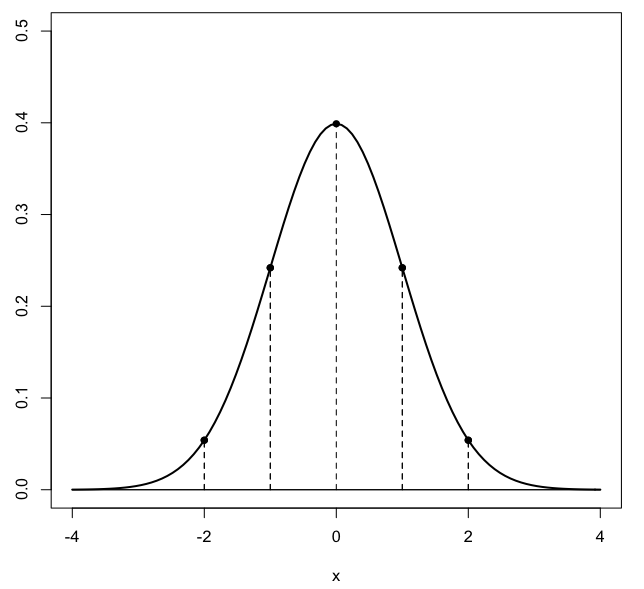
\includegraphics [scale=0.4] {gauss3.png} \end{center}
\begin{document}
\maketitle
\Large
The normal distribution

\url{https://en.wikipedia.org/wiki/Normal_distribution}

is a continuous probability distribution, or a probability density function.  It is also called the "normal" distribution, the "bell curve" and also the Gaussian distribution or Gaussian function.

\begin{center} 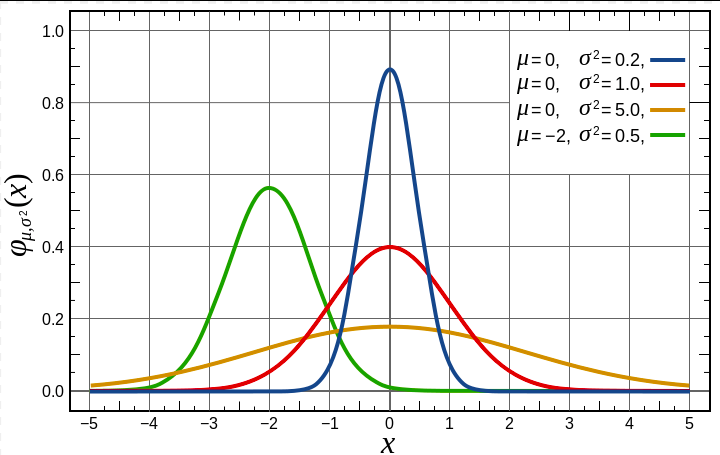
\includegraphics [scale=0.4] {normal-pdf.png} \end{center}

The graphic shows a family of curves or functions, which can be shifted left or right by a value called $\mu$, and rescaled in the $y$-direction by a value called $\sigma$.  When trying to fit a set of data to the normal distribution, the mean ($\mu$) and standard deviation ($\sigma$) or variance ($\sigma^2$) of the data are used to produce a particular curve.

The equation for this distribution is

\[ \frac{1}{k} \int_{-\infty}^{\infty} \  exp \{ -\frac{x - \mu}{2 \sigma^2}) \ dx \]
(the notation $\exp \{ p \}$ is used for $e^p$ when $p$ is unwieldy).

To determine the probability that the random variable lies in the interval $[a,b]$ we compute the integral between these bounds.

The data points can also be adjusted or "centered" to have a mean $\mu = 0$ (by subtracting the mean from each value), and adjusted so that the standard deviation is equal to one (by dividing by $\sigma$).

\url{https://en.wikipedia.org/wiki/Feature_scaling}

In that case, we have the \emph{standard} normal distribution:
\[ \frac{1}{k}  \int e^{-x^2/2} \ dx \]

The constant $k$ ensures that the total area under the curve between the limits $[-\infty,\infty]$  ---the total probability---adds up to 1, as by definition it must for a probability density function.  In other words, $k$ is equal to the value of the integral

\[ k =  \int_{-\infty}^{\infty} \ e^{-x^2/2} \ dx \]
It turns out that 
\[ k = \sqrt{2 \pi} \]

That factor of $\sqrt{\pi}$ is quite amazing.  I want to work through several different proofs of this remarkable fact.  They are taken from:

\url{http://www.math.uconn.edu/~kconrad/blurbs/analysis/gaussianintegral.pdf}

\subsection*{preliminary}
Our goal is to integrate
\[ \int_{-\infty}^{\infty} \ e^{-x^2/2} \ dx \]
Nobody has ever found a way to compute the integral in a general sense, in what is called a "closed form."

\url{https://en.wikipedia.org/wiki/Gaussian_integral}

It turns out that one can compute a value for the integral between the limits $[-\infty,\infty]$ --- over the complete real number line, that is what we're going to do.

But first, notice that this is an even function.  The value for any $x$ is equal to the value for $-x$.  As a result, we can compute 
\[ \int_{0}^{\infty} \ e^{-x^2/2} \ dx \]
and then double the value to obtain what we seek.

Second, the factor of $1/2$ in the exponent can be removed by scaling the variable.  Let
\[ u = \frac{x}{\sqrt{2}}, \ \ \ u^2 = \frac{x^2}{2} \]
\[ \sqrt{2} \ u = x, \ \ \ \sqrt{2} \ du = dx \]
\[ \int e^{-x^2/2} \ dx  = \sqrt{2} \int e^{-u^2} \ du \]

Following the reference article, we define
\[ J = \int_{0}^{\infty} \ e^{-x^2} \ dx \]
so
\[ 2J = \int_{-\infty}^{\infty} \ e^{-x^2} \ dx \]
and
\[ I = \int_{-\infty}^{\infty} \ e^{-x^2/2} \ dx = \sqrt{2} \ (2J) \]
It will turn out that 
\[ 2J = \int_{-\infty}^{\infty} \ e^{-x^2} \ dx = \sqrt{\pi} \]
so, with this notation
\[ I = \sqrt{2 \pi} \]
\[ J = \frac{\sqrt{\pi}}{2} \]
Check this against 
\url{https://en.wikipedia.org/wiki/Gaussian_integral}

For convenience, we usually work with the lower bound of $0$ and then adjust the result.
\subsection*{Poisson}
The best-known proof uses what seems a bit of a trick:  rather than compute $J$ we compute $J^2$ and we do it as a double integral in $xy$-coordinates:
\[ J^2 = \int_{0}^{\infty}  e^{-x^2} \ dx \ \int_{0}^{\infty}  e^{-y^2} \ dy \]
As long as $x$ and $y$ do not depend on each other, this is equivalent to the double integral
\[ \int_{0}^{\infty}  \int_{0}^{\infty}  e^{-x^2} \ e^{-y^2} \ dx \  dy \]

Although it looks tricky, this is basically what Fubini's theorem (that lets us switch the order of integration in a double integral, to first compute either $x$ or $y$)

We do this kind of conversion all the time when working in polar coordinates, where typically $r$ and $\theta$ are independent. Without thinking twice, if $r$ and $\theta$ are independent, we say:

\[ \int_0^{2 \pi} \int_0^R f(r) \ dr \ d \theta = 2 \pi \int f(r) \ dr \]
So now we move forward with the iterated integral:
\[ \int_{0}^{\infty}  \int_{0}^{\infty}  e^{-x^2} \ e^{-y^2} \ dx \  dy = \int_{0}^{\infty}  \int_{0}^{\infty}  e^{-(x^2 + y^2)} \ dx \  dy  \]
It's natural to convert to polar coordinates, remembering that this is an integral over the first quadrant, so we have
\[ \int_0^{\pi/2} \int_0^{\infty} e^{-r^2} \ r \ dr \ d \theta \]
Hopefully, you've seen this before.  The area element in polar coordinates is $r \ dr \ d \theta$.
\begin{center} 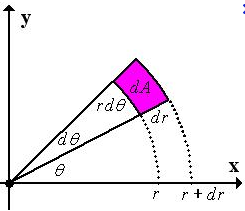
\includegraphics [scale=0.6] {polararea.png} \end{center}
As Strang says "areas always come from multiplying two lengths, and $d\theta$ is not a length." 

The extra $r$ makes the integral easy:
\[ \int_0^{\pi/2} \int_0^{\infty} e^{-r^2} \ r \ dr \ d \theta \]
\[ = \frac{\pi}{2} \  \int_0^{\infty} e^{-r^2} \ r \ dr \]
Save the $\pi/2$ for the moment.  We may guess at the rest:
\[ \frac{d}{dr} \ e^{-r^2} = -2 r \ e^{-r^2} \]
So we need a factor of $-1/2$:
\[ \int_0^{\infty} e^{-r^2} \ r \ dr = -\frac{1}{2} \ e^{-r^2} \ \bigg |_0^{\infty}  = \frac{1}{2} \]
Go back up and pick up $\pi/2$ and the result is $\pi/4$.
\[ J^2 = \frac{\pi}{4} \]
\[ J = \frac{\sqrt{\pi}}{2} \]

\subsection*{Laplace's second method}
We can also do the integral above with single-variable calculus.  Make a change of variables:
\[ x = yt \ \ \ dx = y \ dt \]
\[ J^2 = \int_{0}^{\infty}  \int_{0}^{\infty}  e^{-(x^2 + y^2)} \ dx \  dy  \]
\[ = \int_{0}^{\infty}  \int_{0}^{\infty}  e^{-(y^2t^2 + y^2)} \ y \ dt \  dy  \]
\[ = \int_{0}^{\infty}  \int_{0}^{\infty}  e^{-y^2(t^2 + 1)} \ y \ dt \  dy  \]
\[ = \int_{0}^{\infty} \ [ \  \int_{0}^{\infty}  e^{-y^2(t^2 + 1)} \ y \  dy \ ] \ dt  \]
A standard result is:
\[ \int_0^{\infty} ye^{-ay^2} \  dy = \frac{1}{2a} \ \ \ (a > 0) \]
So our integral is
\[ J^2 = \int_{0}^{\infty} \frac{1}{2(t^2 + 1)} \ dt \]
Do you recognize the inverse tangent?
\[ J^2 = \frac{1}{2} \ \tan^{-1} \ \bigg |_0^{\infty} \]
\[ = \frac{1}{2} \ \frac{\pi}{2} = \frac{\pi}{4} \]

\subsection*{volume integral}
Here is a neat proof based on integrating volumes.

Consider the "bell surface" or Gaussian surface formed by the (unnormalized) function:
\[ z = e^{-(x^2 + y^2)/2} \]

It looks like this:
\begin{center} 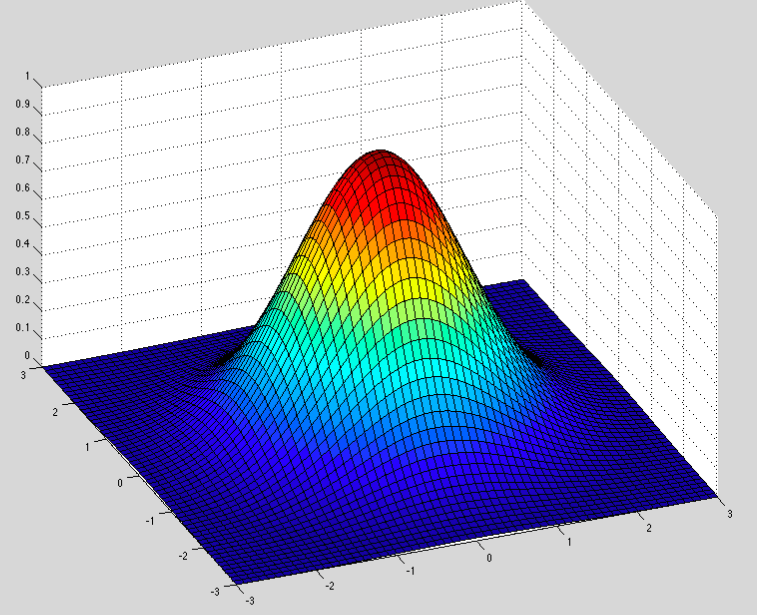
\includegraphics [scale=0.4] {gaussian-surface.png} \end{center}
It's a real bell!

We compute the volume under the surface in two ways.  The first way is by horizontal slices perpendicular to the $z$-axis.

\subsection*{Horizontal}
\[ \int_0^b A(z) \ dz \]
We need an expression for the area of horizontal slices as a function of the height $z$.  What we have now is the inverse function:
\[ z = e^{-(x^2 + y^2)/2} \]
So let's do it:
\[ x^2 + y^2 = -2 \ \ln z \]
The horizontal cross-sections (at $z = c$, where $c$ is a constant), are circles of radius $r$: where
\[ r^2 = x^2 + y^2 = -2 \ \ln z \]

We will fix the upper bound as follows:  the maximum value of $z$ occurs when $x=y=0$ and the exponential is equal to $1$, otherwise the value is less than $1$, so we have that 
\[  b = e^{-(x^2 + y^2)/2} = e^0 = 1 \]
This will be the upper bound on $z$ when we calculate the volume.

So finally, the integral we need starts with $A = \pi r^2$:
\[ A(z) = \pi \ (-2) \ \ln z \]
\[ V = -2 \pi \int_0^1 \ln z \ dz \]
    
Now (leaving the factor of $-2 \pi$ aside for now) that is just:
\[ \int \ln z \ dz = z \ln z - z \]
which is easily verified by differentiating the result.

We need to evaluate this expression between the bounds we set above ($z=0 \rightarrow 1$).

At the lower bound of $z=0$, clearly the second term is zero.
  
The first term is $\ \ln z$.  To evaluate:
\[ \lim_{z \rightarrow 0+}  z \ \ln z  \]

we use L'Hopital's rule:  
\[ z \ \ln z = \frac{z}{1/\ln z} \]

As $z \rightarrow 0+$, the numerator is just zero and the denominator is :$1/-\infty = 0$.

So by the rule, we compute the derivatives:
\[ \frac{1}{1/(1/z)} = z \]
And this limit is equal to zero so we have just zero for the whole expression at the lower bound.

At the upper bound, the first term is zero and the second is equal to $-1$.

Remembering the extra factor, we have finally just $(-2 \pi)(-1) = 2 \pi$.

\subsection*{Vertical}

The other way is vertical slices.  First, recall our definition:
\[ I = \int_{-\infty}^{\infty} e^{-x^2/2} \ dx \]

Again, $I$ is what we're looking for.  It is \textbf{just a number}.  

Our function is
\[ z = e^{-(x^2 + y^2)/2} \]
If we take slices perpendicular to the $x$-axis (with $x =$ constant for any particular slice), the area of each slice is
\[ A(x) = \int_{-\infty}^{\infty} e^{-(x^2 + y^2)/2} \ dy \]
since  $x$ is a constant we have
\[ = e^{-x^2/2} \ \int_{-\infty}^{\infty} e^{-y^2/2} \ dy = e^{-x^2/2} \ I \]

Now we add up all the little slices to find the volume, which is
\[  V =  \int_{-\infty}^{\infty} I e^{-x^2/2} \ dx \]
but $I$ is just a number, so
\[  =  I \int_{-\infty}^{\infty} e^{-x^2/2} \ dx \]
\[ = I^2 \]

Now we have two different expressions for the same volume, which must be equal to each other.  Thus:
\[ 2 \pi = I^2 \]
\[ I = \sqrt{2 \pi} \]

\subsection*{Gamma function}
And last, a method using the Gamma function.

The Gamma function is:
\[  \Gamma(x) = \int_0^{\infty} t^{x-1} e^{-t} \ dt \]

A bit more about it here:

\url{https://en.wikipedia.org/wiki/Gamma_function}

For integer $n$
\[  \Gamma(n) = (n-1)! \]
Here is one important property of the gamma function that is easily proved using integration by parts:
\[ \Gamma (x+1) = x \Gamma(x) \]
The gamma function is like the factorial, but it generalizes to non-integer values of $x$, and it's offset by $1$.

A second property:
\[ \frac{\Gamma(x) \Gamma(y)}{\Gamma (x+y)} = \int_0^1 t^{x-1}(1-t)^{y-1} \ dt \]
This is actually the Beta function (see note at the end).

\subsection*{Trick with x = 1/2}
In any case, using this last equation, set
\[  x = y = \frac{1}{2} \]
then
\[ [ \ \Gamma(\frac{1}{2}) \ ]^2 = \int_0^1 \frac{1}{\sqrt{t(1-t)}} \ dt \]
Now, from the standard definition of the gamma function:
\[ \Gamma(x) = \int_0^{\infty} t^{x-1} e^{-t} \ dt \]
\[ \Gamma(\frac{1}{2}) = \int_0^{\infty} \frac{1}{\sqrt{t}} e^{-t} \ dt \]
Do a change of variable
\[ \sqrt{t} = x, \ \ \ t = x^2, \ \ \ dt = 2 x \ dx \]
and then
\[ \Gamma(\frac{1}{2}) = \int_0^{\infty} \frac{1}{x} e^{-x^2} \ 2 x \ dx \]
\[ = 2 \int_0^{\infty} e^{-x^2} \ dx \]
\[ = 2 J \]
So 
\[ 4J^2 = \  [ \ \Gamma(\frac{1}{2}) \ ]^2 = \int_0^1 \frac{1}{\sqrt{t(1-t)}} \ dt \]

To do this integral, substitute:
\[  t = \sin^2 \theta \]
\[  dt = 2 \sin \theta \cos \theta \ d \theta \]
\[ \sqrt{t(1-t)} = \sqrt{t} \ \sqrt{1-t} = \sin \theta \cos \theta \]
So the integral is simply 
\[ \int \frac{2 \sin \theta \cos \theta \ d \theta}{\sin \theta \cos \theta} = 2 \int d \theta = 2 \theta \]
!!

What are the bounds?
\[ t = \sin^2 \theta = 0 \Rightarrow \theta = 0 \]
\[ t =  \sin^2 \theta = 1 \Rightarrow \theta = \frac{\pi}{2} \]
The final value is just $2 \theta = \pi$.  (Notice, we have shown that 
\[ \Gamma(\frac{1}{2}) \ ]^2 = \pi \]
\[ \Gamma(\frac{1}{2}) \  = \sqrt{\pi} \]
    
So:
\[ 4J^2 = \int_0^1 \frac{1}{\sqrt{t(1-t)}} \ dt = \pi \]
 \[ J = \frac{\sqrt{\pi}}{2} \]

\url{http://www.math.uconn.edu/~kconrad/blurbs/analysis/gaussianintegral.pdf}

\subsection*{Beta function}
The Beta function $B(x,y)$ is 
\[ B(x,y) = \int_0^1 t^{x-1}(1-t)^{y-1} \ dt \]
It turns out that $B(x,y)$ is equal to 
\[ B(x,y) = \frac{\Gamma(x) \Gamma(y)}{\Gamma (x+y)} \]
For more about this see

\url{https://en.wikipedia.org/wiki/Beta_function}

Here is the derivation shown in wikipedia.  Recall that:
\[ \Gamma(x) = \int_0^{\infty} e^{-u} \ u^{x-1} \ du \]
so
\[ \Gamma(x) \ \Gamma(y) = \int_0^{\infty} e^{-u} \ u^{x-1} \ du \ \int_0^{\infty} e^{-v} \ v^{y-1} \ dv \]
\[ = \int_0^{\infty}  \ \int_0^{\infty} e^{-u-v} \ u^{x-1} \ v^{y-1} \ du \   dv \]
We make a change of variables as follows:
\[ u = zt \]
\[ v = z(1-t) \]
so the integral becomes
\[ = \iint e^{-z} \ (zt)^{x-1} \  (z(1-t))^{y-1} \ dt \ dz \]
times a factor which is the Jacobian (normally abbreviated $J$, but here I will use $j$):

For convenience define
\[ u_z= \frac{\partial u}{\partial z} = t \]
\[ u_t = \frac{\partial u}{\partial t} = z \]
\[ v_z= \frac{\partial v}{\partial z} = 1-t \]
\[ v_t = \frac{\partial v}{\partial t} = -z \]
and
\[ j = 
\begin{vmatrix}
u_z & u_t \\
v_z & v_t
\end{vmatrix} = u_z v_t - u_t v_z \]
\[ = -zt - z(1-t) = -z \]
Remembering to use the \emph{absolute value} of the determinant

\url{https://en.wikipedia.org/wiki/Jacobian_matrix_and_determinant}

we have
\[ = \iint \ e^{-z} (zt)^{x-1} \  (z(1-t))^{y-1} \ z \ dt \ dz \]
\[ = \iint \ e^{-z} z^{x-1} \ z^{y-1} \ z \ dz \  (1-t)^{y-1} \  t^{x-1} \ dt \]
\[ = \iint \ e^{-z} z^{x+y-1} \ dz \ t^{x-1} \ (1-t)^{y-1} \ dt \]
A key feature here is that the bounds are now $t = 0 \rightarrow 1$, while $z = 0 \rightarrow \infty$.  (I'm not completely sure of the justification for this).
\[ = \int_{z=0}^{\infty} e^{-z} z^{x + y - 1} \ dz  \ \int_{t=0}^1 t^{x-1} (1-t)^{y-1} \ dt \]
\[ = \Gamma(x+y) \ B(x,y) \]
Hence
\[ \Gamma(x) \Gamma(y) =  \Gamma(x+y) \ B(x,y) \]
and the result follows.
\end{document}  